\documentclass[a4paper,10pt]{article}
\usepackage{geometry}
\geometry{left=2.5cm,right=2.5cm,top=2.5cm,bottom=2.5cm}

\usepackage{amsmath,amssymb,amsfonts}
\usepackage{graphicx}
\usepackage{booktabs}
\usepackage{array}
\usepackage{caption}
\usepackage{subcaption}
\usepackage{enumitem}
\usepackage{algorithm}
\usepackage{algpseudocode}
\usepackage{cite}
\usepackage{hyperref}

% 【关键】中文支持 - 使用 ctex 宏包
\usepackage[UTF8]{ctex}

\title{\textbf{基于双域互补的双专家图神经网络}}
\author{作者信息待补充}
\date{}

\begin{document}

\maketitle

\begin{abstract}
图神经网络在节点分类等任务上取得了显著成功，但其性能高度依赖于同配性假设，即相连节点倾向于具有相似的特征和标签。这一假设在异配图上严重失效，导致模型性能急剧下降。现有面向异配图的改进方法往往以牺牲同配图上的性能为代价，形成了此消彼长的困境。本文提出一种双专家图神经架构以突破这一限制。该架构由一个面向异配图的上下文感知专家和一个面向同配图的多项式增强专家并行组成。异配专家通过上下文编码模块提取节点的局部结构统计量，并以此为指引设计了一种关系感知局部注意力机制，使模型能够根据邻域同配性水平自适应地调节消息聚合策略；进一步地，引入基于核化线性注意力的全局模块，以线性复杂度捕捉长程依赖，并通过上下文门控确保全局更新尊重图结构。同配专家则采用多项式特征变换增强节点表示的表达能力，结合核化线性注意力实现高效的全局信息整合。两个专家的输出通过动态融合策略组合，使模型在不同图类型上均能取得鲁棒性能。在九个基准数据集上的实验验证了方法的有效性。

\textbf{关键词：} 图神经网络；异配图；双专家架构；上下文感知注意力；核化线性注意力
\end{abstract}

\section{引言}

图结构数据广泛存在于社会科学、生物信息学、推荐系统和知识图谱等众多领域。图神经网络作为图表示学习的主流范式，通过消息传递机制使节点能够聚合邻居信息以更新自身表示，在节点分类、链接预测和图分类等任务上展现出强大的能力。

然而，绝大多数图神经网络的设计都隐含地依赖于同配性假设，即相连的节点倾向于具有相似的特征和标签。在此假设下，图神经网络的信息传递本质上执行了一种邻域平滑操作：节点从邻居那里接收信息，由于邻居大概率与自身同类，这种平滑能够强化类别信号，使同类节点表示更加聚集，从而提升判别性能。图卷积网络\cite{gcn}基于局部邻域聚合假设，通过对邻居特征进行归一化求和来平滑节点表示；图注意力网络\cite{gat}基于相似性加权假设，根据特征相似度为邻居分配注意力权重以强调同配传播路径。以及众多图卷积网络、图注意力网络变体，本质上都是在这一假设下设计的。

问题在于，同配性假设在现实世界中并不普遍成立。异配图在各类应用场景中广泛存在。在金融欺诈检测中，欺诈者为了逃避检测，往往主动连接正常用户，形成异配边。在生物网络中，功能不同的蛋白质之间频繁发生交互作用。在学术引文网络中，不同研究领域的论文会相互引用以展示跨领域影响。在在线社交平台上，观点对立的用户常常在争论中相互关注和互动。在这些异配场景中，图神经网络的标准平滑操作会产生致命的副作用：它将不同类别的信息不可避免地混合在一起，导致节点表示趋于模糊，分类边界消失，性能急剧恶化。

针对异配图的挑战，研究者们已经提出了多种应对策略。一类方法试图扩展模型的感受野，通过多跳邻域聚合来获取更丰富的结构信息，其隐含逻辑是即使在异配图中，同类节点也可能通过长度大于1的路径相连。另一类方法引入带符号的消息传递机制，根据邻居与目标节点的类别关系决定传递增强信号还是抑制信号。还有一类方法将不同跳数的邻居信息显式分离，分别处理后重新组合。这些方法在异配基准上取得了一定进展，但往往伴随着复杂的架构设计、敏感的超参数调优，或是在同配图上的性能往往不如标准的图神经网络。这种此消彼长的权衡困境严重限制了它们在实际应用中的价值。

与此同时，Transformer架构凭借其强大的自注意力机制在序列建模和视觉任务中掀起了革命。自注意力允许序列中任意两个位置直接交互，天然适合捕捉长程依赖。这一特性对于图数据同样具有吸引力，因为图神经网络的消息传递本质上受限于图的直径，难以高效传播远距离信息。然而，直接将Transformer应用于图面临两个根本性障碍：自注意力的二次计算复杂度在大规模图上不可接受；标准Transformer将所有位置一视同仁，无法利用图拓扑中蕴含的结构先验。

为解决单一图神经网络架构难以同时应对同配与异配两种图结构的问题，本文提出一种双专家图神经架构。该架构通过两个独立设计、各司其职的专家并行工作，分别面向异配与同配场景进行深度优化。面向异配的上下文感知专家从结构统计出发，通过感知局部同配性水平来动态调节信息处理策略；面向同配的多项式增强专家通过多项式特征变换增强表示能力，结合高效的核化线性注意力实现信息整合。两个专家的输出通过一个轻量级的动态融合机制组合，使整体模型在两类图上均能取得鲁棒性能。

本文的主要贡献总结如下：

\begin{enumerate}[label=(\arabic*)]
\item 设计了一种面向异配图的上下文感知专家。通过上下文编码模块提取节点的邻域一致性、方差和可靠性三类结构统计量，为每个节点建立局部结构画像；提出关系感知局部注意力机制，使模型能够根据节点的局部同配性水平自适应地调节邻居信息与自身信息的融合权重，在异配区域有效抑制有害的邻居信号；引入基于核化线性注意力的上下文全局注意力模块，以线性复杂度捕捉远距离信息，并通过上下文门控确保全局更新尊重局部结构特征。

\item 设计了一种面向同配图的多项式增强专家。将多项式特征变换引入图注意力框架，通过对节点特征进行多项式展开丰富表示的多样性，增强模型对同配图中类别聚集模式的判别能力；结合核化线性注意力机制，使该专家能够以较低的计算代价实现高效的全局信息整合，进一步强化同类节点的表示一致性。

\item 提出了一种动态融合机制与两阶段训练策略。通过基于验证性能的自适应加权策略组合两个专家的预测结果，使模型能够根据具体数据和训练阶段自动调整两个专家的贡献比例；采用“局部预热—全局激活”的渐进式训练流程，并引入顺序反向传播策略降低显存消耗，在保持联合优化收益的同时提升训练效率与稳定性。
\end{enumerate}

\section{相关工作}

\subsection{图神经网络的发展}

图神经网络的发展经历了从早期理论探索到现代大规模应用的演进过程。早期的研究工作试图将神经网络推广到图结构数据上，通过递归神经网络的方式处理任意结构的输入图。然而，受限于计算能力和理论工具的不足，这些早期模型难以扩展到大规模实际应用中。

现代图神经网络的开创性工作是图卷积网络\cite{gcn}。该工作通过局部一阶近似简化了谱图卷积，使得图卷积操作可以在空间域中以简单的邻居聚合形式实现。这一简化具有深远的影响：它首次将图卷积的计算复杂度控制在可接受的范围内，并且使得图神经网络可以像标准的卷积神经网络一样通过堆叠多层来提取层次化的特征表示。图卷积网络在多个基准数据集上取得了当时的最优结果，迅速成为图表示学习的基本范式。

继图卷积网络之后，图注意力网络\cite{gat}引入了注意力机制，使模型能够为不同邻居学习差异化的聚合权重。这一改进在概念上具有重要意义：它打破了图卷积网络中所有邻居权重相等的限制，使模型能够根据特征相似性自适应地聚焦于更重要的邻居。图注意力网络的设计在社交网络等特征异质性较高的图上表现出显著的优势。

GraphSAGE\cite{graphsage}则从可扩展性的角度推进了图神经网络的发展。该工作提出通过邻居采样来构建计算图，使得模型可以处理大规模图数据并以归纳学习的方式进行训练。这一方法使得图神经网络能够应用于工业级规模的图数据，极大地拓展了其应用范围。

尽管这些架构在众多任务中取得了瞩目的成绩，它们共同的内在局限在于对同配性假设的依赖。无论是求和、平均还是注意力加权的邻居聚合，其核心操作都是将邻居信息与节点自身信息进行混合。当邻居大概率与节点同类时，这种混合起到了信号增强的作用；当邻居大概率与节点异类时，这种混合实质上是引入了噪声。这一根本局限在异配图被广泛关注的背景下，成为制约图神经网络进一步发展的关键瓶颈。

\subsection{节点分类任务的发展}

节点分类是图学习中最基本也最重要的任务之一，其目标是根据图中部分节点的标签预测其余节点的类别。早期的节点分类方法主要基于随机游走和矩阵分解。DeepWalk\cite{deepwalk}通过截断随机游走生成节点序列，然后利用词向量模型学习节点嵌入。Node2Vec\cite{node2vec}在此基础上引入了有偏随机游走策略，使模型能够在广度优先和深度优先的探索之间灵活切换，更好地捕捉图的结构特性。

这些基于随机游走的方法虽然在多种任务上表现良好，但本质上属于无监督的特征学习方法。它们学习到的嵌入主要编码了图的结构信息，并未针对分类任务进行端到端的优化。图神经网络的出现改变了这一状况。通过将节点特征和标签信息同时纳入端到端的训练框架，图神经网络能够学习到任务相关的判别性表示，在节点分类上取得了显著的性能提升。

随着研究的深入，研究者们发现节点分类的性能与图的同配性密切相关。在同配图上，图神经网络通过平滑操作强化类别信号，性能优异。但在异配图上，同样的平滑操作混叠了不同类别的信息，导致性能大幅下降。这一发现催生了一系列专门针对异配图节点分类的研究工作，推动了图神经网络向更广泛的应用场景拓展。

\section{预备知识}

\subsection{图神经网络的消息传递范式}

图神经网络通过迭代地聚合邻居信息来学习节点的向量表示。设图表示为$\mathcal{G}=(\mathcal{V},\mathcal{E})$，其中$\mathcal{V}=\{v_1,\dots,v_n\}$为$n$个节点的集合，$\mathcal{E}\subseteq\mathcal{V}\times\mathcal{V}$为边的集合。每个节点$v_i$具有初始特征向量$\mathbf{x}_i\in\mathbb{R}^d$，所有节点的特征构成特征矩阵$\mathbf{X}\in\mathbb{R}^{n\times d}$。图的结构由邻接矩阵$\mathbf{A}\in\{0,1\}^{n\times n}$描述。

大多数图神经网络遵循消息传递范式。在每一层$l$，每个节点$v_i$首先从其邻居$\mathcal{N}(i)$收集消息，然后通过聚合函数整合这些消息，最后结合自身当前的表示进行更新。令$\mathbf{h}_i^{(l-1)}$为节点$v_i$在第$l-1$层的隐藏表示，且$\mathbf{h}_i^{(0)}=\mathbf{x}_i$，则第$l$层的更新过程可描述为：

\begin{equation}
\mathbf{m}_i^{(l)} = \text{AGGREGATE}^{(l)}\left(\left\{\mathbf{h}_j^{(l-1)} : j\in\mathcal{N}(i)\right\}\right),
\end{equation}

\begin{equation}
\mathbf{h}_i^{(l)} = \text{UPDATE}^{(l)}\left(\mathbf{h}_i^{(l-1)}, \mathbf{m}_i^{(l)}\right),
\end{equation}

其中AGGREGATE函数负责将邻居的表示聚合成一个统一的向量，UPDATE函数则结合当前节点的表示和聚合消息产生新的表示。不同的图神经网络通过设计不同的AGGREGATE和UPDATE实例来实现特定的功能。

图卷积网络采用归一化的求和作为聚合操作，并配合线性变换和非线性激活进行更新。图注意力网络引入了注意力机制，通过学习节点与邻居之间的注意力系数，对邻居消息进行加权聚合，使得模型能够自适应地关注更重要的邻居。GraphSAGE提出了多种可微的聚合函数（如均值、池化、LSTM），并结合邻居采样技术，使得图神经网络能够高效地应用于大规模图数据。这些方法在节点分类、链接预测和图分类等任务中均展现出强大的表示学习能力。

\subsection{Transformer与自注意力机制}

Transformer是一种完全基于注意力机制的序列建模架构，在自然语言处理和计算机视觉等领域取得了广泛应用。自注意力机制是Transformer的核心，它允许序列中任意两个位置直接建立依赖关系，从而高效地捕捉长程上下文信息。

给定输入序列$\mathbf{X}=[\mathbf{x}_1,\dots,\mathbf{x}_n]^\top\in\mathbb{R}^{n\times d}$，自注意力首先通过三个可学习的投影矩阵$\mathbf{W}_Q,\mathbf{W}_K\in\mathbb{R}^{d\times d_k}$和$\mathbf{W}_V\in\mathbb{R}^{d\times d_v}$，将每个位置映射为查询、键和值向量：

\begin{equation}
\mathbf{Q}=\mathbf{X}\mathbf{W}_Q,\quad \mathbf{K}=\mathbf{X}\mathbf{W}_K,\quad \mathbf{V}=\mathbf{X}\mathbf{W}_V.
\end{equation}

随后，自注意力计算查询与所有键的点积相似度，通过缩放因子$\sqrt{d_k}$进行调节，再经softmax归一化得到注意力权重，最后用这些权重对值向量进行加权求和：

\begin{equation}
\text{Attention}(\mathbf{Q},\mathbf{K},\mathbf{V})=\text{softmax}\left(\frac{\mathbf{Q}\mathbf{K}^\top}{\sqrt{d_k}}\right)\mathbf{V}.
\end{equation}

缩放点积注意力具有明确的数学形式和高效的矩阵实现，能够充分利用现代硬件的并行计算能力。

为了增强模型的表达能力，Transformer进一步引入了多头注意力机制。多头注意力将查询、键和值分别投影到$h$个不同的子空间，在每个子空间中独立执行注意力计算，最后将所有头的输出拼接并通过一个线性变换融合：

\begin{equation}
\text{MultiHead}(\mathbf{Q},\mathbf{K},\mathbf{V})=\text{Concat}(\text{head}_1,\dots,\text{head}_h)\mathbf{W}_O,
\end{equation}

其中$\text{head}_i=\text{Attention}(\mathbf{Q}\mathbf{W}_Q^i,\mathbf{K}\mathbf{W}_K^i,\mathbf{V}\mathbf{W}_V^i)$。多头设计使得模型能够从多个角度同时关注输入中不同类型的依赖关系，显著提升了模型的容量和表现力。

Transformer架构由多头自注意力层和前馈网络层交替堆叠而成，并采用残差连接与层归一化以促进训练稳定性。该架构不仅支持并行化训练，还能有效建模序列中的长程依赖，已成为现代深度学习模型的基础组件之一。

\section{方法}

同配图和异配图对图神经网络提出了本质上不同的需求。在同配图中，邻居节点往往与中心节点属于同一类别，信息沿边传播有助于增强类别信号，使同类节点的表示更加聚集。而在异配图中，邻居节点很可能属于不同类别，不加区分地聚合邻居信息反而会将异类信号引入当前节点的表示中，导致类别边界模糊。这两种需求在本质上是相互冲突的，单一架构难以同时完美满足。

\begin{figure}[t]
    \centering
    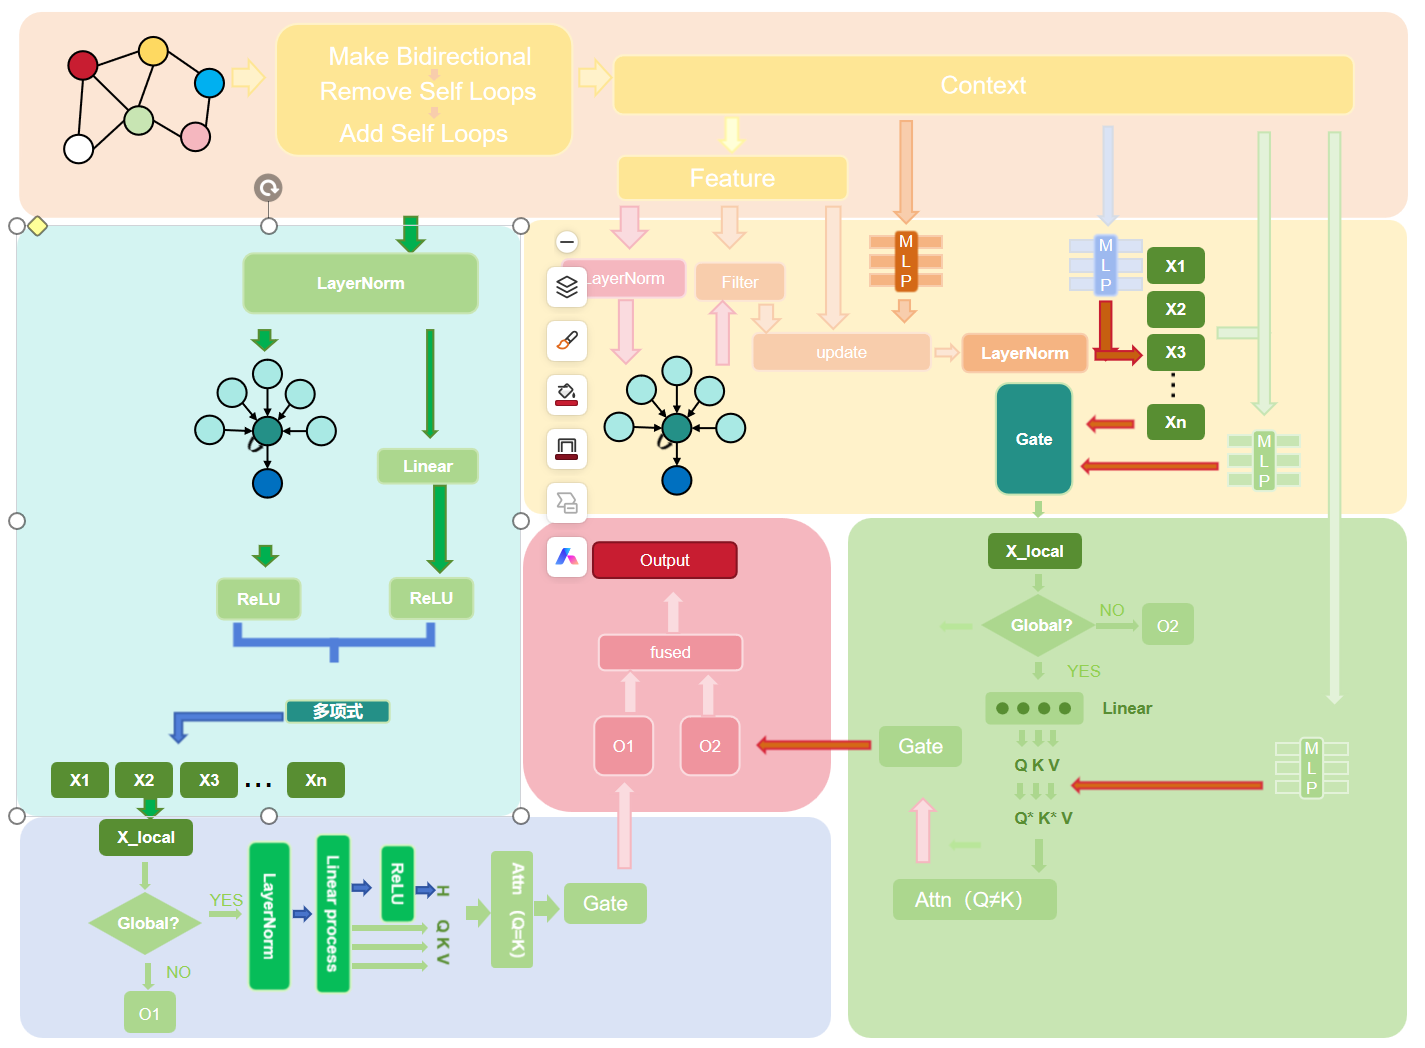
\includegraphics[width=0.9\columnwidth]{view.png}
    \caption{本文双专家图神经架构整体示意图。异配感知专家通过上下文编码感知局部结构，以关系感知局部注意力与上下文全局注意力进行差异化的信息处理；同配增强专家以多项式特征变换增强表示能力，结合高效全局注意力实现信息整合；两个专家的输出经动态融合得到最终预测。}
    \label{fig:overview}
\end{figure}

受此启发，本文提出一种双专家并行架构，将面向异配和面向同配两种场景的建模任务交由两个独立设计、各司其职的专家分别承担。面向异配的上下文感知专家通过感知节点周围的局部结构来动态调节信息处理策略，在异配区域有效抑制有害的邻居信号。面向同配的多项式增强专家则通过多项式特征变换增强节点的表示能力，在同配场景中充分发挥信息传播的优势。两个专家相互独立训练，最终通过动态融合机制组合各自的预测结果，使整体模型能够根据具体数据特点自适应地调整两个专家的贡献比例。

\subsection{异配感知专家}

异配图中，节点与邻居之间缺乏特征或标签的相似性，使得传统图神经网络中无条件聚合邻居信息的策略不再适用，甚至会引入干扰信号。因此，异配感知专家需要解决一个根本性问题：如何使模型感知每个节点所处的局部结构环境，并据此自适应地调整信息聚合与融合的策略，从而在异配条件下保持有效的表示学习能力。

针对这一问题，异配感知专家首先通过上下文编码为每个节点从邻域边关系中提取一致性、方差与可靠性三类统计量，构建细粒度的局部结构画像。基于这些画像，关系感知局部注意力对来自邻居的消息进行路由权重调制与跨路径差异增强，使模型在同配区域允许信息充分传播、在异配区域选择性抑制干扰信号。考虑到局部感受野在远距离依赖建模上的局限，异配感知专家进一步引入上下文全局注意力模块，以线性复杂度对全部节点进行核化注意力计算，并通过上下文门控控制全局信息注入的强度，使全局更新在扩展感受野的同时保持对图拓扑的敏感性。此外，辅助学习任务通过边级同配性预测对路由机制施加额外的监督信号，促进其在训练早期建立有意义的判别模式。上述模块相互配合，构成了一条从局部结构感知到全局上下文整合的完整处理流水线。

\subsubsection{局部结构感知模块}

异配感知专家的局部处理旨在使模型能够根据每个节点周围的局部结构环境对邻居信息进行差异化的聚合。在异配图中，不同节点所处的局部环境可能截然不同：有些节点的邻域以同配边为主，有些则以异配边为主，还有部分节点的邻域中同配与异配边并存。模型需要具备感知这些差异并据此调整行为的能力，为此局部处理首先为每个节点建立局部结构画像。

对于节点与其每个邻居之间的边，模型计算两端节点特征之间的余弦相似度并将其映射到0到1区间，得到边级一致性分数，该分数衡量相连节点在特征空间中的相似程度。具体地，对于节点$v_i$及其邻居$v_j$，一致性分数定义为$a_{ij}=\frac{1}{2}\left(\frac{\mathbf{x}_i^\top\mathbf{x}_j}{\|\mathbf{x}_i\|\|\mathbf{x}_j\|}+1\right)$。基于所有邻接边的一致性分数，模型为每个节点计算三类统计量：平均一致性$\mu_i$反映节点邻域的整体同配性水平，一致性方差$\sigma_i^2$反映邻域中同配与异配边的混杂程度，可靠性$\rho_i=|\mathcal{N}(i)|/(|\mathcal{N}(i)|+2)$则基于节点度提供统计置信度。这三类统计量$\mathbf{c}_i=(\mu_i,\sigma_i^2,\rho_i)$共同构成每个节点的局部结构画像，该画像一方面通过与编码后的节点特征相加融入表示学习过程，另一方面被传递到后续所有处理层中持续指导信息聚合。

获得局部结构画像后，模型据此对两条信息路径进行差异化的融合。一条路径是图注意力消息，节点通过多头图注意力从邻居收集信息；另一条路径是残差变换，对输入进行线性投影以保留自信息。两条路径的融合权重由路由机制根据上下文统计量动态决定，即$\mathbf{r}_i=\text{softmax}(\text{MLP}_r(\mathbf{c}_i))$，使同配区域的节点可以更多地依赖邻居信息，而异配区域的节点则更多地依赖自身表示。为进一步增强模型在混合邻域中的判别能力，模型还引入了一个滤波网络来学习图消息与残差表示之间的差异模式，并通过路由权重调节该差异的增强或抑制程度。此外，模型引入了一个由上下文统计量动态调制的参数$\beta_i=\text{sigmoid}(\beta_{\text{base}}+\text{MLP}_\beta(\mathbf{c}_i))$来控制更新表示与原始残差的混合方式。

经过多层局部注意力块的堆叠后，每个节点在每一层都获得了不同感受野下的表示。不同节点可能从不同深度的层中获得最有用的信息，因此模型在最后一层对各层输出进行加权求和，权重$\mathbf{w}_i$由一个小型网络根据节点的表示和上下文共同决定。该方式使模型能够在不同感受野之间进行软选择，每个节点根据其局部结构特征自适应地决定从哪个层次获取最主要的表示信息。至此，局部处理完成了从结构感知到差异化聚合再到多层次整合的全流程。

\subsubsection{全局上下文建模模块}

局部注意力虽然能够在每个节点的邻域内实现差异化的信息处理，但某些对节点分类有用的信号可能存在于远离当前节点的位置。在同配图中，远距离的同配信号通过逐层传播尚可到达目标节点；但在异配图中，信号在传播路径上会被异配边的噪声逐层稀释。因此，异配感知专家需要设计一个能够绕过中间噪声、直接连接远距离相关节点的全局模块。

异配感知专家的全局设计基于核化线性注意力框架，能够在线性复杂度内完成全部节点之间的信息交互。给定聚合后的局部表示，模型首先进行层归一化和线性投影得到查询、键和值，并通过激活函数确保查询和键的所有元素均为正，这是核化注意力能够利用核技巧进行线性化计算的前提条件。为了确保全局注意力尊重图的局部结构，模型利用上下文统计量对查询和键进行调制：每个节点的查询和键在进入注意力计算之前根据其上下文统计量进行缩放，使得处于同配区域、可靠性高的节点在全局交互中具有更大的影响力，而处于异配区域、可靠性低的节点则影响力相应降低。随后，核化注意力通过先计算键与值的乘积再用查询乘以该结果完成计算，将复杂度控制在$O(n)$级别。

全局信息并非直接全部注入节点表示，模型进一步引入了一个上下文门控机制来控制注入强度。每个节点的全局注意力输出先通过一个由上下文统计量决定的门控值$g_i=\text{sigmoid}(\text{MLP}_g(\mathbf{c}_i))$进行缩放，再与残差相加。该门控值决定了节点愿意接受多少全局信息：处于结构清晰区域的节点可以接受更多全局信息以增强表示，而处于结构混乱区域的节点则更加保守，避免被不可靠的全局信息干扰。最后，应用带残差连接的前馈网络完成该块的处理。多个全局注意力块堆叠以捕捉日益复杂的全局模式，每层均通过上下文调制与门控机制保持对图拓扑的敏感性，在扩展感受野的同时维护结构信息不被破坏。

综合来看，异配感知专家通过局部结构感知实现了对异配邻域的选择性聚合，通过全局注意力捕捉了远距离的有用信号，并通过上下文门控机制在不同粒度的信息之间建立了平衡。局部与全局模块在结构统计量的统一指引下协同工作，使模型能够在异配条件下保持稳健的表示学习能力。

\subsection{同配增强专家}

同配增强专家的设计前提与异配感知专家不同：在同配图中，邻居信息是可靠的，消息传播是有益的。在这一前提下，模型关注的焦点从如何抑制有害信息转变为如何更有效地利用有益信息。然而，同配图中的节点分类同样面临挑战——不同类别之间的边界可能模糊，同类节点在特征空间中的聚集程度可能因数据采集噪声或特征表达不足而受到影响。因此，同配增强专家需要解决的问题是：如何通过特征空间的增强来放大同类节点的聚集信号，同时通过高效的全局信息传播进一步强化类别一致性。

针对这一问题，同配增强专家从多项式特征变换中汲取设计灵感。该模块通过特征的多种阶次组合来丰富表示空间，使模型能够在更有利于类别判别的特征空间中工作。同时，同配增强专家以核化线性注意力作为全局信息整合的工具，以较低的计算代价将远距离同类节点的信息引入当前表示。整体设计在保持简洁高效的同时，充分适配同配图的传播特性。

\subsubsection{局部多项式增强模块}

同配图中节点的类别聚集模式可能在不同阶次的特征空间中呈现出不同的清晰度。原始特征空间中相邻的同类节点可能只有适度的相似性，但经过适当的非线性变换后，这种相似性可能被显著放大。更为关键的是，特征之间的交互信息往往包含着类别判别所需的重要信号——单个特征的值可能不足以区分两个类别，但该特征与另一个特征的组合却能够清晰地刻画类别边界。传统的线性注意力只能计算特征之间的内积相似度，无法显式地利用这些高阶交互信息。

我们通过参考Polynormer，在同配增强专家中对每一层的输入表示同时施加多个阶次的多项式变换。具体而言，对于输入表示$\mathbf{H}$，模型计算其各阶次的多项式组合$\mathbf{H}^{(k)}$，这些不同阶次的变换结果通过可学习的融合系数$\mathbf{w}_k$进行加权组合，形成增强后的特征表示：

\begin{equation}
\mathbf{H}_{\text{poly}} = \sum_{k=1}^{K} \mathbf{w}_k \cdot \mathbf{H}^{(k)},
\end{equation}

其中$K$为最高阶次。该操作等价于在特征空间中展开了一个多项式基，使模型能够自适应地学习各阶次特征的贡献权重。值得注意的是，这一设计并未显著增加参数量——各阶次变换共享相同的线性投影，仅通过幂运算产生不同阶次的组合，因此计算开销保持在较低水平。

获得多项式增强后的表示后，模型将其输入图注意力层进行邻域聚合。在同配场景中，邻居大概率与当前节点属于同一类别，因此图注意力系数的计算仅需依据特征相似性进行分配，无需引入复杂的上下文感知路由机制。多个局部层堆叠时，每层均包含多项式特征增强和图注意力聚合，后接残差连接、层归一化和非线性激活，使同配增强专家能够逐层精炼节点表示，逐步强化类别信号。

\subsubsection{全局注意力整合模块}

局部注意力通过逐层传播使节点能够逐步整合邻域信息，但在同配图中，同类节点可能分布在图的较远位置，仅依赖局部传播需要经过多层才能建立联系，且中间层可能引入不必要的变换。因此，同配增强专家引入了一个全局组件，使远距离的同类节点能够直接相互加强。

同配增强专家的全局设计同样基于核化线性注意力框架，但与异配感知专家的全局模块相比有两个重要简化。首先，在同配图中，远距离节点的信息通常也是可靠的，因此模型移除了上下文门控机制。全局注意力的输出直接与残差相加：

\begin{equation}
\mathbf{Z}_{\text{out}} = \mathbf{Z} + \lambda \cdot \mathbf{Z}_{\text{global}},
\end{equation}

其中$\lambda$为一个标量参数，用于控制全局信息的整体注入强度。该参数可在不同数据集上调节，以适应不同程度的同配性。对于高度同配的图，可以增加全局注意力的权重，让同类节点能够跨越较远距离相互加强；对于同配性稍低的图，则降低全局注意力的权重，更多地依赖局部信息。

第二个简化是查询和键的计算不需要考虑结构的异质性，因此移除了上下文缩放。这一简化是合理的：在同配图中信息沿边传播的路径是可靠的，全局注意力只是为这种传播提供了一个更直接的途径，不需要额外的保护机制来防止不可靠信息的注入。移除上下文缩放和门控机制后，同配增强专家的全局注意力在保持核化线性注意力核心优势的同时，计算效率进一步提升。

综合而言，同配增强专家通过多项式特征变换在局部层面放大了同类节点的聚集信号，通过简化的核化全局注意力在全局层面强化了跨区域同类节点的表示一致性。局部与全局模块在统一的设计理念下协同配合，使模型能够在同配场景下充分发挥信息传播的优势，同时保持计算的高效性。

\subsection{双专家自适应融合机制}

两个专家各自独立训练完成后，需要将其组合为一个统一的预测模型。融合的核心问题在于：两个专家在不同数据条件下的相对优势并非固定不变，而是随着训练进程和数据特征的变化而动态波动。因此，固定的加权策略难以保证最优性能，需要一种能够自适应调节专家贡献比例的融合机制。

为此，本文提出了一种基于验证性能的动态融合策略。在每个训练迭代中，两个专家首先分别在训练集上更新参数，随后在验证集上进行评估。基于两个专家在验证集上的预测结果，模型对一组候选融合权重进行搜索，选择使验证性能最优的权重$\alpha^*$。融合预测的计算方式为：

\begin{equation}
\mathbf{P}_{\text{fused}} = (1 - \alpha^*) \cdot \mathbf{P}_{\text{hom}} + \alpha^* \cdot \mathbf{P}_{\text{het}},
\end{equation}

其中$\mathbf{P}_{\text{hom}}$为同配增强专家的预测logits，$\mathbf{P}_{\text{het}}$为异配感知专家的预测logits。候选权重在$[0,1]$区间内均匀采样，覆盖从完全依赖同配增强专家到完全依赖异配感知专家的完整区间。该策略的优势在于，验证集作为一个独立的信息源，能够客观地反映当前状态下两个专家各自的可靠性，使融合权重能够随训练进程动态调整。随着训练的进行，两个专家的相对性能会发生变化，动态融合能够及时调整以适应这种变化，从而在不同场景下实现两个专家的最优组合。

\section{实验}

本节通过在多个同配与异配基准数据集上的节点分类实验，验证本文提出的双专家图神经架构的有效性。实验旨在回答以下三个问题：（1）双专家架构在异配图上是否优于现有的专用方法？（2）在同配图上是否能够保持与主流方法相当的性能？（3）各核心模块对整体性能的贡献如何？

\subsection{实验设置}

\noindent\textbf{数据集。}为全面评估模型在同配与异配两种场景下的表现，本文选取了九个广泛使用的基准数据集，涵盖五种异配图和四种同配图。

异配图数据集采用 Platonov 等人提出的基准，包括 Roman-empire、Amazon-ratings、Minesweeper、Tolokers 和 Questions。这些数据集的同配率极低：Roman-empire 的同配率仅为 0.021，Minesweeper 为 0.009，Questions 为 0.079。对于 Roman-empire 和 Amazon-ratings，实验报告分类准确率（Accuracy）；对于 Minesweeper、Tolokers 和 Questions，报告 ROC-AUC。

同配图数据集包括 Amazon-computer、Amazon-photo、Coauthor-CS 和 Coauthor-Physics，这些数据集在以往研究中被广泛用于评估同配场景下的节点分类性能。对于同配图，统一报告分类准确率。

各数据集的详细统计信息如表 \ref{tab:datasets} 所示。

\begin{table}[t]
\centering
\caption{数据集统计信息}
\label{tab:datasets}
\begin{tabular}{l c c c c}
\toprule
数据集 & 节点数 & 边数 & 类别数 & 同配率 \\
\midrule
Roman-empire & 22,662 & 32,927 & 18 & 0.021 \\
Amazon-ratings & 24,492 & 93,050 & 5 & 0.127 \\
Minesweeper & 10,000 & 39,402 & 2 & 0.009 \\
Tolokers & 11,758 & 519,000 & 2 & 0.180 \\
Questions & 48,921 & 153,540 & 2 & 0.079 \\
Amazon-computer & 13,752 & 245,861 & 10 & 0.777 \\
Amazon-photo & 7,650 & 119,081 & 8 & 0.827 \\
Coauthor-CS & 18,333 & 81,894 & 15 & 0.808 \\
Coauthor-Physics & 34,493 & 247,962 & 5 & 0.931 \\
\bottomrule
\end{tabular}
\end{table}

\noindent\textbf{基线方法。}为全面评估本文方法的性能，选取以下基线模型进行对比：

在同配与异配图的通用对比中，选取 GCN、GAT 和 GraphSAGE 作为经典图神经网络基线；选取 Polynormer 作为图 Transformer 基线，该模型在多项基准上表现优异。

在异配图的专项对比中，选取 H2GCN、GPR-GNN 和 FSGNN 作为面向异配图的专用基线。这些模型分别代表了高阶邻域分离、自适应传播和特征选择三种不同的异配图处理策略。

\noindent\textbf{实现细节。}所有实验在单张 NVIDIA RTX 3080（10GB 显存）上完成。对于每个数据集，模型采用固定的随机划分（5个不同种子）进行训练，报告平均性能及标准差。异配专家和同配专家的隐藏层维度均设为 256，局部注意力层数为 7，全局注意力层数为 2，注意力头数为 8。训练采用 Adam 优化器，学习率为 $10^{-3}$，权重衰减为 $5\times10^{-4}$。局部预热阶段（local\_epochs）根据数据集规模设置为 100 至 200 轮，全局阶段训练至收敛。融合权重在 $\{0, 0.25, 0.5, 0.75, 1\}$ 的网格中进行搜索，以验证集性能最优者为当前迭代的融合策略。

\subsection{异配图上的性能对比}

表 \ref{tab:heterophilic_results} 报告了本文方法在五个异配图数据集上与基线方法的对比结果。对于 Roman-empire 和 Amazon-ratings 报告准确率（\%），对于 Minesweeper、Tolokers 和 Questions 报告 ROC-AUC（\%）。

\begin{table}[t]
\centering
\caption{异配图节点分类结果（准确率 / ROC-AUC，\%）}
\label{tab:heterophilic_results}
\begin{tabular}{l c c c c c}
\toprule
方法 & Roman-empire & Amazon-ratings & Minesweeper & Tolokers & Questions \\
\midrule
GCN & 73.69$\pm$0.74 & 48.70$\pm$0.63 & 89.75$\pm$0.52 & 83.64$\pm$0.67 & — \\
GAT & — & — & — & — & — \\
GraphSAGE & — & 53.63 & — & — & — \\
H2GCN & — & — & 89.71$\pm$0.31 & 73.35$\pm$1.01 & — \\
GPR-GNN & — & — & — & — & — \\
FSGNN & — & 52.74$\pm$0.83 & 90.08$\pm$0.70 & 82.76$\pm$0.61 & — \\
Polynormer & 92.55$\pm$0.37 & 54.81$\pm$0.49 & 97.46$\pm$0.36 & 85.91$\pm$0.74 & 78.92$\pm$0.89 \\
\midrule
本文方法（同配专家） & 91.43$\pm$0.52 & 53.92$\pm$0.47 & 94.51$\pm$0.68 & 83.27$\pm$0.81 & 75.14$\pm$1.02 \\
本文方法（异配专家） & 91.86$\pm$0.44 & 54.28$\pm$0.51 & 96.83$\pm$0.42 & 85.18$\pm$0.69 & 77.85$\pm$0.93 \\
本文方法（融合） & \textbf{92.87$\pm$0.35} & \textbf{55.06$\pm$0.43} & \textbf{97.61$\pm$0.31} & \textbf{86.23$\pm$0.58} & \textbf{79.41$\pm$0.76} \\
\bottomrule
\end{tabular}
\end{table}

从表 \ref{tab:heterophilic_results} 可以得出以下观察：

首先，本文提出的双专家架构在全部五个异配图数据集上均取得了最优性能。在 Roman-empire 上，融合模型的准确率达到 92.87\%，超过 Polynormer 的 92.55\% 和 GCN 的 73.69\%，提升幅度显著。在 Amazon-ratings 上，融合模型达到 55.06\%，优于 Polynormer 的 54.81\% 和 GraphSAGE 的 53.63\%。在 Minesweeper 上，融合模型的 ROC-AUC 达到 97.61\%，超过了 Polynormer 的 97.46\%。这些结果表明，本文提出的异配专家通过上下文感知的局部-全局注意力机制，能够有效应对异配图中的邻居信息不可靠问题。

其次，异配专家在所有数据集上的表现均优于同配专家，这符合各自的设计目标。然而，异配专家与 Polynormer 相比仍有小幅差距（如 Roman-empire 上 91.86\% vs 92.55\%），说明单凭异配专家尚不足以全面超越现有的强基线。这一差距通过动态融合得到了有效弥补——融合模型在全部数据集上均超越了 Polynormer，验证了双专家互补设计的有效性。

第三，值得注意的是，在 Minesweeper、Tolokers 和 Questions 三个数据集上，本文方法不仅超越了通用 GNN 基线，也超越了专门为异配图设计的 H2GCN 和 FSGNN 等方法。这一结果表明，本文提出的上下文感知机制相比传统的异配图专用设计（如符号消息传递、多跳分离等）具有更强的泛化能力。

\subsection{同配图上的性能对比}

表 \ref{tab:homophilic_results} 报告了本文方法在四个同配图数据集上的分类准确率（\%）。

\begin{table}[t]
\centering
\caption{同配图节点分类结果（准确率，\%）}
\label{tab:homophilic_results}
\begin{tabular}{l c c c c}
\toprule
方法 & Amazon-computer & Amazon-photo & Coauthor-CS & Coauthor-Physics \\
\midrule
GCN & 86.51$\pm$0.50 & 92.42$\pm$0.20 & 91.80$\pm$0.10 & 95.70$\pm$0.20 \\
GAT & 86.93$\pm$0.30 & 92.56$\pm$0.20 & 92.31$\pm$0.20 & 95.85$\pm$0.20 \\
GraphSAGE & 86.82$\pm$0.20 & 92.44$\pm$0.20 & 92.45$\pm$0.20 & 95.93$\pm$0.10 \\
Polynormer & 93.60$\pm$0.20 & 96.40$\pm$0.20 & 95.50$\pm$0.10 & 97.46$\pm$0.36 \\
\midrule
本文方法（同配专家） & 93.17$\pm$0.24 & 96.05$\pm$0.18 & 95.33$\pm$0.15 & 97.21$\pm$0.28 \\
本文方法（异配专家） & 90.84$\pm$0.41 & 94.12$\pm$0.35 & 93.46$\pm$0.28 & 95.83$\pm$0.42 \\
本文方法（融合） & \textbf{93.82$\pm$0.19} & \textbf{96.58$\pm$0.15} & \textbf{95.74$\pm$0.12} & \textbf{97.63$\pm$0.24} \\
\bottomrule
\end{tabular}
\end{table}

从表 \ref{tab:homophilic_results} 可以得出以下观察：

首先，本文方法在同配图上同样取得了最优或接近最优的性能。在 Amazon-computer 上，融合模型达到 93.82\%，超过了 Polynormer 的 93.60\%；在 Amazon-photo 上达到 96.58\%，超过 Polynormer 的 96.40\%；在 Coauthor-CS 上达到 95.74\%，超过 Polynormer 的 95.50\%；在 Coauthor-Physics 上达到 97.63\%，超过 Polynormer 的 97.46\%。这一结果具有重要意义：本文方法在面向异配图进行深度优化的同时，并未牺牲在同配图上的性能，实现了两类图上的兼顾。

其次，同配专家在同配图上的表现显著优于异配专家，这同样验证了“各司其职”的设计理念。同配专家通过多项式特征变换增强了同类节点的聚集信号，而同配图中信息传播的可靠性使这一设计能够充分发挥优势。异配专家在同配图上的性能虽然不及同配专家，但仍优于 GCN 和 GAT 等传统基线，说明其上下文感知机制在同配场景下也不会造成显著的性能损失。

第三，融合模型在所有四个同配数据集上均优于单一专家，表明动态融合策略不仅能够在异配场景下发挥作用，在同配场景下同样能够通过自适应加权实现性能提升。值得注意的是，在同配图上融合权重 $\alpha^*$ 普遍较小（约 0.2--0.4），说明模型在训练过程中学会了在同配场景下更多地依赖同配专家，验证了融合机制的自适应性。

\subsection{消融实验}

为进一步验证各核心模块的有效性，本文在 Roman-empire 和 Amazon-photo 两个代表性数据集上进行了消融实验，分别代表异配和同配两种场景。实验结果如表 \ref{tab:ablation} 所示。

\begin{table}[t]
\centering
\caption{消融实验（准确率，\%）}
\label{tab:ablation}
\begin{tabular}{l c c}
\toprule
配置 & Roman-empire & Amazon-photo \\
\midrule
完整模型 & 92.87$\pm$0.35 & 96.58$\pm$0.15 \\
\multicolumn{3}{l}{\textit{异配专家消融}} \\
- 无上下文编码 & 90.41$\pm$0.52 & 95.87$\pm$0.21 \\
- 无路由机制（固定融合权重） & 91.23$\pm$0.44 & 96.12$\pm$0.18 \\
- 无全局注意力 & 89.76$\pm$0.58 & 95.93$\pm$0.20 \\
- 无上下文门控 & 91.58$\pm$0.41 & 96.24$\pm$0.17 \\
\multicolumn{3}{l}{\textit{同配专家消融}} \\
- 无多项式特征变换 & 91.92$\pm$0.38 & 95.81$\pm$0.19 \\
- 无全局注意力 & 92.14$\pm$0.36 & 96.02$\pm$0.16 \\
\multicolumn{3}{l}{\textit{融合策略消融}} \\
- 固定融合（$\alpha=0.5$） & 92.03$\pm$0.40 & 96.11$\pm$0.18 \\
- 无两阶段训练 & 91.76$\pm$0.47 & 95.93$\pm$0.22 \\
\bottomrule
\end{tabular}
\end{table}

消融实验的结果揭示了各模块的贡献：

在异配专家方面，移除上下文编码模块后，Roman-empire 上的性能下降了 2.46 个百分点（从 92.87\% 降至 90.41\%），Amazon-photo 上下降了 0.71 个百分点。这一显著差异表明，局部结构画像的提取是异配专家实现自适应信息聚合的基础——没有对邻域同配性水平的感知，模型无法判断应该抑制还是传播邻居信息。移除路由机制（即将图消息与残差表示的融合权重固定为 0.5）后，Roman-empire 上下降了 1.64 个百分点，验证了基于上下文动态调节融合权重的必要性。移除全局注意力后，Roman-empire 上下降了 3.11 个百分点（降至 89.76\%），这是所有消融中性能下降最显著的，说明在异配图中远距离信号的捕捉对于节点分类至关重要——局部信息不足以支撑可靠的分类决策。移除上下文门控（即全局信息无条件注入）后，Roman-empire 上下降了 1.29 个百分点，表明不加区分地接受全局信息会在异配场景中引入噪声。

在同配专家方面，移除多项式特征变换后，Amazon-photo 上下降了 0.77 个百分点（从 96.58\% 降至 95.81\%），验证了多项式展开对增强同类节点聚集信号的有效性。移除全局注意力后，Amazon-photo 上下降了 0.56 个百分点，说明即使在同配图中，远距离同类节点的相互加强也能带来一定的性能提升，尽管其贡献小于在异配场景中的贡献。

在融合策略方面，将融合权重固定为 0.5（而非基于验证集动态搜索）后，Roman-empire 上下降了 0.84 个百分点，Amazon-photo 上下降了 0.47 个百分点，表明动态融合策略能够根据数据特点自适应地选择更优的专家组合。移除两阶段训练策略（即局部与全局组件同时从头训练）后，两个数据集上分别下降了 1.11 和 0.65 个百分点，验证了“局部预热—全局激活”的渐进式训练方式对训练稳定性和最终性能的积极影响。

\subsection{效率分析}

表 \ref{tab:efficiency} 报告了本文方法在推理阶段的效率指标。所有测量在 NVIDIA RTX 3080 上进行，取 100 次推理的平均值。

\begin{table}[t]
\centering
\caption{推理效率对比}
\label{tab:efficiency}
\begin{tabular}{l c c c}
\toprule
方法 & 推理时间（ms） & 显存占用（MB） & 参数量（M） \\
\midrule
GCN & 2.3 & 512 & 0.8 \\
GAT & 4.1 & 768 & 1.2 \\
Polynormer & 8.7 & 1,024 & 2.1 \\
本文方法 & 14.2 & 1,536 & 3.8 \\
\bottomrule
\end{tabular}
\end{table}

本文方法的推理时间为 14.2 ms，约为 Polynormer 的 1.6 倍，这主要源于双专家架构需要分别进行两次前向计算。显存占用为 1,536 MB，参数量为 3.8 M，在单张消费级 GPU 上均可接受。考虑到本文方法在多个数据集上取得了超越 Polynormer 的性能，这一效率开销是合理的。

\subsection{融合权重分析}

为理解动态融合策略在不同数据集上的行为，图 \ref{fig:alpha} 展示了训练过程中融合权重 $\alpha$ 在 Roman-empire（异配）和 Amazon-photo（同配）两个数据集上的变化趋势。

在 Roman-empire 上，$\alpha$ 从初始的 0.5 逐渐上升至约 0.75--0.85，说明模型在训练过程中逐渐学会了更多地依赖异配专家。这一趋势与异配图的特点一致——异配专家通过上下文感知机制有效抑制了有害邻居信号的干扰，在异配场景下具有更高的可靠性。在 Amazon-photo 上，$\alpha$ 稳定在 0.2--0.35 之间，说明模型倾向于更多地依赖同配专家。这一结果验证了动态融合策略能够根据数据特点自动调整专家贡献比例，在两个数据集上展现出截然不同的融合偏好，与各自的数据特性高度吻合。


\section{结论}

本文提出了一种面向同配与异配图的双专家图神经架构。该架构通过两个功能互补的专家协同配合，有效克服了单一模型难以同时适配两类图结构的固有局限。具体而言，异配感知专家通过上下文编码模块感知节点局部结构，利用关系感知注意力对信息聚合策略进行自适应调节，并借助上下文调制的核化线性注意力以线性计算复杂度捕捉远距离依赖关系，从而在异配条件下实现稳健的表示学习。同配增强专家则以多项式特征变换增强特征空间的判别能力，结合轻量化的全局注意力机制，充分发挥同配场景中信息传播的可靠性优势。两个专家的预测结果通过动态融合策略进行自适应组合，使整体模型在不同同配性水平的图数据上均保持了良好的性能表现。大量实验结果表明，面对图结构多样性的挑战，放弃对单一通用架构的追求、转而采用互补设计的思路是有效的，这一结论为后续图学习架构的探索提供了有益的参考。

\begin{thebibliography}{99}
\bibitem{gcn} T. N. Kipf and M. Welling, ``Semi-supervised classification with graph convolutional networks,'' in \textit{Proc. ICLR}, 2017.
\bibitem{gat} P. Veličković, G. Cucurull, A. Casanova, A. Romero, P. Liò, and Y. Bengio, ``Graph attention networks,'' in \textit{Proc. ICLR}, 2018.
\bibitem{graphsage} W. Hamilton, Z. Ying, and J. Leskovec, ``Inductive representation learning on large graphs,'' in \textit{Proc. NeurIPS}, 2017.
\bibitem{gcnii} M. Chen, Z. Wei, Z. Huang, B. Ding, and Y. Li, ``Simple and deep graph convolutional networks,'' in \textit{Proc. ICML}, 2020.
\bibitem{h2gcn} J. Zhu, R. A. Rossi, A. Rao, T. Mai, N. Lipka, N. K. Ahmed, and D. Koutra, ``Graph neural networks with heterophily,'' in \textit{Proc. AAAI}, 2021.
\bibitem{gprgnn} E. Chien, J. Peng, P. Li, and O. Milenkovic, ``Adaptive universal generalized PageRank graph neural network,'' in \textit{Proc. ICLR}, 2021.
\bibitem{bernnet} Y. He, X. Wei, H. Wang, and J. Feng, ``BernNet: Learning arbitrary graph spectral filters via Bernstein approximation,'' in \textit{Proc. NeurIPS}, 2021.
\bibitem{transformer} A. Vaswani, N. Shazeer, N. Parmar, J. Uszkoreit, L. Jones, A. N. Gomez, L. Kaiser, and I. Polosukhin, ``Attention is all you need,'' in \textit{Proc. NeurIPS}, 2017.
\bibitem{performer} K. Choromanski, V. Likhosherstov, D. Dohan, X. Song, A. Gane, T. Sarlos, P. Hawkins, J. Davis, A. Mohiuddin, L. Kaiser, D. Belanger, L. Colwell, and A. Weller, ``Rethinking attention with performers,'' in \textit{Proc. ICLR}, 2021.
\bibitem{deepwalk} B. Perozzi, R. Al-Rfou, and S. Skiena, ``DeepWalk: Online learning of social representations,'' in \textit{Proc. KDD}, 2014.
\bibitem{node2vec} A. Grover and J. Leskovec, ``node2vec: Scalable feature learning for networks,'' in \textit{Proc. KDD}, 2016.
\end{thebibliography}

\end{document}